%
% tsunami.tex -- 
%
% (c) 2011 Prof Dr Andreas Mueller, Hochschule Rapperswil
%

\section{Application: Wave propagation on a sphere or the tsunami of 2011}
\index{Tsunami}
On march 11 2011, an magnitude 9 earthquake in the japanese sea,
somtimes also referred to as the Sendai earthquake, triggered a 
tsunami that devastated large areas of the coast of the japanese
Fukushima province.
More than 15000 people were killed and multiple nuclear plants
were impacted, of which the the Fukushima-Daichi plant with a
a partial core meltdown was the most serious.
Tsunamis are waves triggered by earthquakes.
They are hardly noticeable in the open ocean and travel quite fast
but grow dramatically when the approach shallow waters near the coast.
The propagation of waves can modelled with a wave equation as has
been presented in chapter~\ref{chapter:examples}, but usually with
a propagation speed dependent on the depth of the ocean.
Figures \ref{tsunamiausbreitung} and \ref{tsunamienergie}
show the propagation of the wave caused by the Sendai earthquake
computed with the help of a computer.
It is obvious that the topography of the sea floor has a significant
influence on the propagation.

This makes a manual computation of the wave propagation almost
impossible, we would have to completely model the ocean floor and
the details of the coastline.
As a simplified model, we can try to understand the propagation of a
wave on an ocean covering a sphere with constant depth.

\begin{figure}
\begin{center}
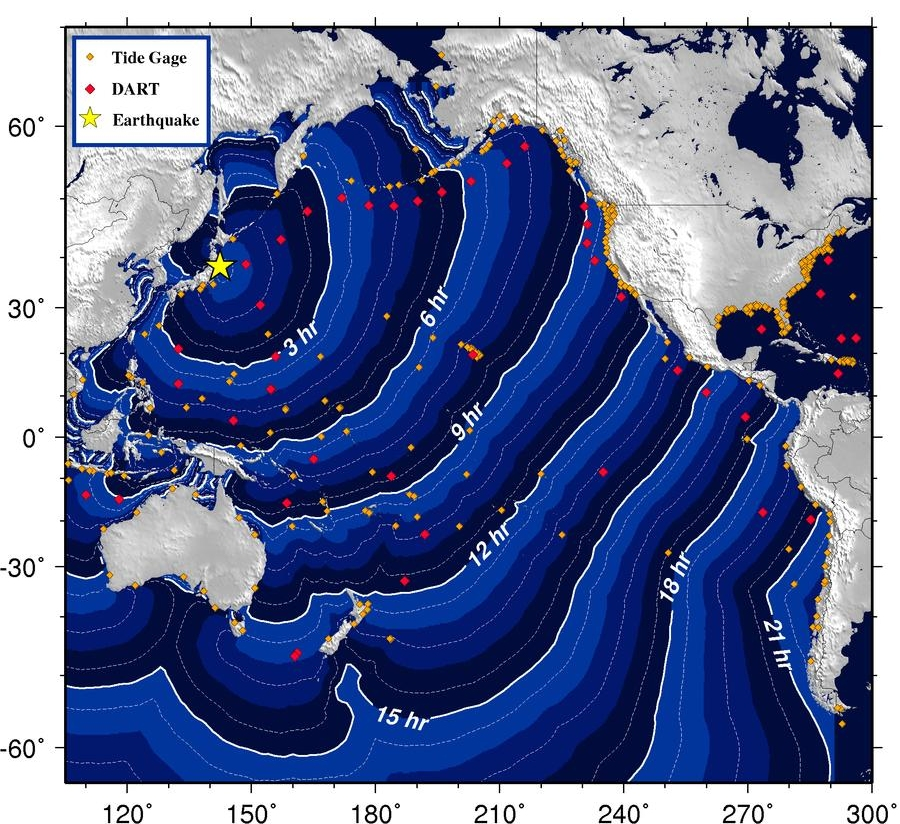
\includegraphics[width=\hsize]{../common/graphics/sendainoaa}
\end{center}
\caption{
Propagation of the tsunami caused by the Sendai earthquake on march 11 2011
based on a simulation by NOAA.
Hawai and other islands reduce the depth and thus the speed of propagation
of the wave.
Also apparent the shadowing of the wave due to obstacles like New Zealand.
\label{tsunamiausbreitung}}
\end{figure}

\begin{figure}
\begin{center}
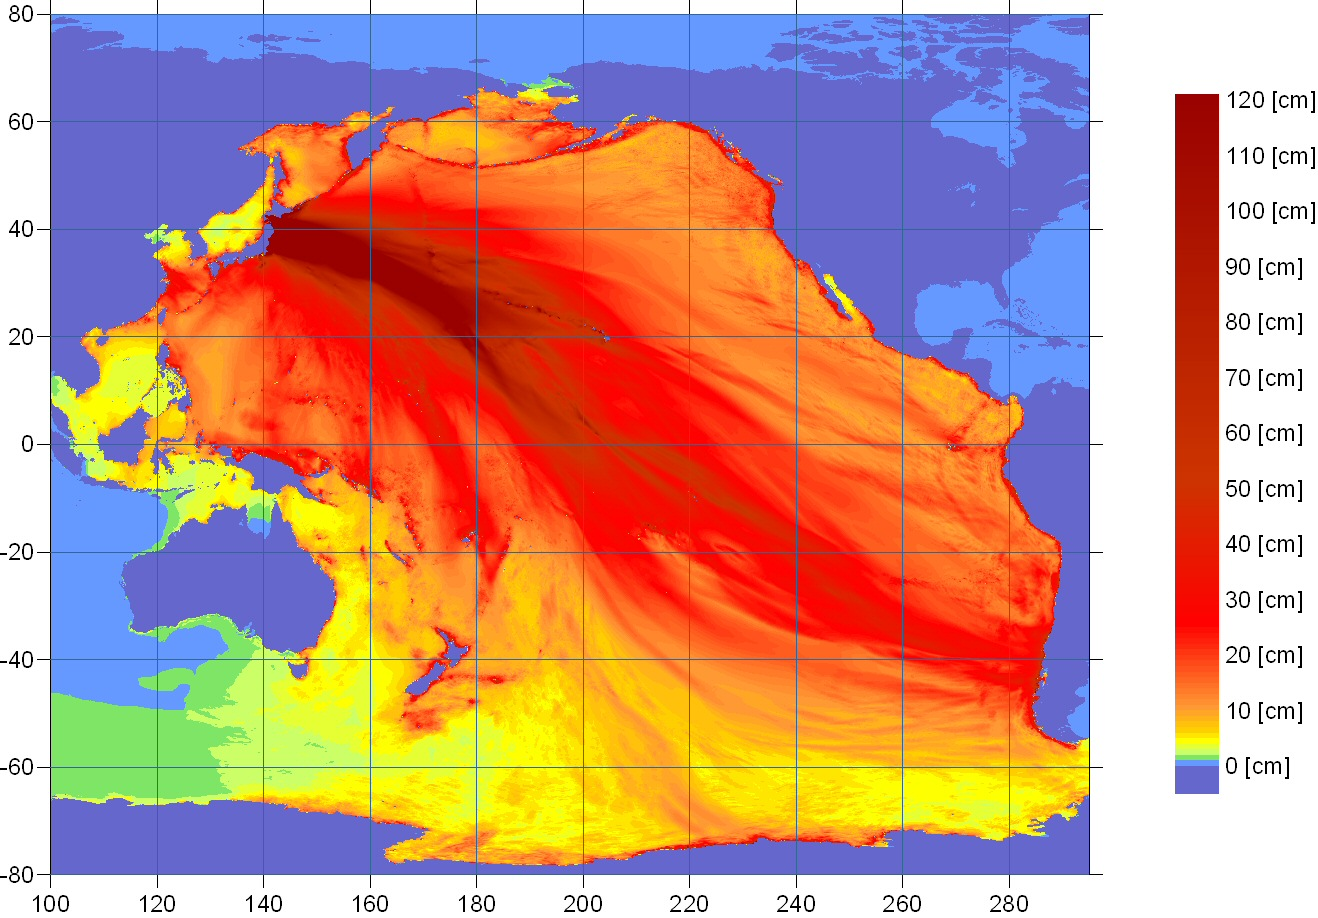
\includegraphics[width=\hsize]{../common/graphics/sendaienergy}
\end{center}
\caption{
Amplitude of the tsuname of march 11 2011.
Note that the great circles along which the waves propagate are mapped
to S-shaped durves.
Close to the coast the amplitude increases because of the reduced depth
and thus reduced velocity.
\label{tsunamienergie}}
\end{figure}

\subsection{Coordinates and boundary conditions}
We are interested in a wave originating in a single point, the
epicenter of the earthquake.
The solution in the idealized situation will necessarily be rotationally
symmetric around the axis through the epicenter.

We use spherical coordinates $(r,\vartheta,\varphi)$.
$\vartheta$ is the latitude measured from the north pole which will
also be the epicenter.
$\varphi$ is the longitude, a rotationally symmetric wave will not
depend on $\varphi$.
We can also neglect the $r$, as we consider only what happens at the
surface.
We therefore set $r=1$.

We are looking for a function
$u(t,\vartheta)$ satisfying initial conditions
\begin{align*}
u(0,\vartheta)&=F(\vartheta)\\
\frac{\partial}{\partial t}u(0,\vartheta)&=G(\vartheta).
\end{align*}

\subsection{Wave equation on the surface of a sphere}
The wave equation on the surface of a sphere can be obtained
by restricting the three dimensional wave equation
\[
\frac1{c^2} \frac{\partial^2}{\partial t^2}u =\Delta u.
\]
to the surface of the sphere.
We assume that units are chosen so that $c=1$, which amounts
to setting the time unit to time it takes for the wave to travel
one earth radius.

We can assume that the units are chosen in such a way that 
the $c=1$.
This can be accomplished by taking the radius of the earth as the
unit of length and the time it takes for the wave to travel one
earth radius as the unit of time.

The Laplacian must be expressedin spherical coordinates,
\[
\Delta u
=
\frac1{r^2} \frac{\partial}{\partial r}r^2\frac{\partial}{\partial r}u
+
\frac1{r^2\sin\vartheta}
\frac{\partial}{\partial\vartheta}
\sin\vartheta
\frac{\partial}{\partial\vartheta}
u
+
\frac1{r^2\sin^2\vartheta}\frac{\partial^2}{\partial\varphi^2}u
=
\frac1{\sin\vartheta}
\frac{\partial}{\partial\vartheta}
\sin\vartheta
\frac{\partial}{\partial\vartheta}
u
\]
The wave equation now turns into
\begin{equation}
\frac{\partial^2u}{\partial t^2}=
\frac1{\sin\vartheta}
\frac{\partial}{\partial\vartheta}
\sin\vartheta
\frac{\partial}{\partial\vartheta}
u=0.
\label{tsunami-gleichung}
\end{equation}

\subsection{Separation}
For the solution of the wave equation \eqref{tsunami-gleichung}
we now use the separation ansatz:
\[
u(t,\vartheta)=T(t)\Theta(\vartheta),
\]
and substitute it into the differential equation:
\[
T''(t)\Theta(\vartheta)=
T(t)
\frac1{\sin\vartheta}
\frac{d}{d\vartheta}
\sin\vartheta
\frac{d}{d\vartheta}\Theta(\vartheta)
\]
Since we are looking for a solution that does not vanish identically,
we may assume that $T(t)$ and $\Theta(\vartheta)$ only vanish in isolated
points so that we can divide by $T(t)\Theta(\vartheta)$ almost everywhere.
This allows us to separate the variables we were looking for:
\begin{equation}
\frac{T''(t)}{T(t)}
=
\frac1{\Theta(\vartheta)}
\frac1{\sin\vartheta}
\frac{d}{d\vartheta}
\sin\vartheta
\frac{d}{d\vartheta}\Theta(\vartheta).
\label{tsunami-separiert}
\end{equation}
The left hand side depends only on $t$, the right hand side only on
$\vartheta$.
This implies that the both sides are constant, giving us two coupled equations
\begin{align}
T''(t)&=mT(t)
\label{tsunami:zeitabh}
\\
\frac1{\sin\vartheta}
\frac{d}{d\vartheta}
\sin\vartheta
\frac{d}{d\vartheta}\Theta(\vartheta)
&=m\Theta(\vartheta).
\label{tsunami:winkelabh}
\end{align}
We now have to figure out which values $m$ for which both equations
can have solutions with reasonable boundary conditions which we
then can use to superimpose arbitrary solutions.

\subsection{Time dependence}
The time dependence equation \eqref{tsunami:zeitabh} is an ordinary
oscillation equation.
The solutions must have oscillatory character, which is only possible
for $m<0$.
The general solution then becomes
\[
T_m(t)=a_m\cos\sqrt{-m}t+b_m\sin\sqrt{-m}t
\]

\subsection{Angular dependency}
The differential equation \eqref{tsunami:winkelabh} for $\Theta$
is a little bit unwieldy.
By replacing $\Theta(\vartheta)$ by a function $y(x)$
using the substitution $x=\cos\vartheta$.
The derivative with respect to $\vartheta$ can be converted into
a derivative with respect to $x$ using the chain rule:
\[
\frac{d}{d\vartheta}\Theta(\vartheta)
=\frac{dy(x)}{dx}\frac{dx}{d\vartheta}
=-\sin\vartheta \frac{d}{dx} y(x)
\]
Using this in the differential equation, we obtain
\begin{align*}
\frac1{\sin\vartheta}
(-\sin{\vartheta})\frac{d}{dx}\sin\vartheta (-\sin\vartheta)
\frac{d}{dx}y(x)
&=
\frac{d}{dx}\sin^2\vartheta\frac{d}{dx}y(x)\\
&=
\frac{d}{dx}(1-\cos^2\vartheta)\frac{d}{dx}y(x)\\
&=
\frac{d}{dx}(1-x^2)\frac{d}{dx}y(x).
\end{align*}
The function we are looking for is therefore a solution of the
differential equation
\begin{equation}
\frac{d}{dx}(1-x^2)\frac{d}{dx}y(x)
=
my(x)
\label{tsunamieigenwertproblem}
\end{equation}
The function $y(x)$ must be defined in the entire interval $[-1,1]$.
This isn't automatic, as one can see already in the case $m=0$.
In that case, the differential equation can be integrating 
twice:
\begin{align*}
\frac{d}{dx}(1-x^2)\frac{d}{dx}y(x)&=0\\
(1-x^2)\frac{d}{dx}y(x)&=C\\
\frac{d}{dx}y(x)&=\frac{C}{1-x^2}\\
y(x)&=C\int\frac{dx}{1-x^2}\\
&=\frac{C}2\int\frac{dx}{1-x}+\frac{C}2\int\frac{dx}{1+x}\\
&=-\frac{C}2\log(1-x)+\frac{C}2\log(1+x) +D\\
&=\frac{C}2\log\frac{1+x}{1-x} + D
\end{align*}
At both interval ends, the function increases beyond bounds
unless $C=0$.

Polynomials would certainly be well defined on the whole interval,
so we attempt to solve the equation with a function of the form
\[
y(x)=a_0+a_1+a_2x^2+\dots a_nx^n.
\]
Substituting this in the differential equation and keeping only
terms of degree $n$, i.~e.~with $x^n$, we get  $ma_nx^n$
on the right side of \eqref{tsunamieigenwertproblem}.
On the left side we get
\[
-\frac{d}{dx}x^2\frac{d}{dx}a_nx^n
=
-\frac{d}{dx}x^2na_nx^{n-1}
=
-\frac{d}{dx}na_nx^{n+1}
=
-n(n+1)a_nx^n
\]
It follows that $m=-n(n+1)$, the equation \eqref{tsunamieigenwertproblem}
can only be solved with a polynomial of degree $n$ for precisely those
values ov $m$.
The differential equation now becomes
\begin{equation}
\frac{d}{dx}(1-x^2)\frac{d}{dx}y(x)+n(n+1)y(x)=0
\label{legendredgl}
\end{equation}

\subsection{Legendre polynomials}
The differential equation \eqref{legendredgl} is known as the differential
equation for the legendre polynomials.
The legendre polynomail $P_n(x)$ is a polynomial solution of
\eqref{legendredgl} with boundary condition $P_n(1)=1$.
However, this condition does not yet uniquely determine the function.
The additional condition is imposed that the polynomials also be
orthogonal in the sense that
\[
\int_{-1}^1 P_k(x)P_l(x)\,dx=0\quad\text{für $k\ne l$}.
\]
This allows to construct a theory similar to fourier theory for
approximation of functions in the interval $[-1,1]$.
This then determines the polynomials uniquely.

The first six Legendre polynomials are
\begin{align*}
P_0(x)&=1\\
P_1(x)&=x\\
P_2(x)&=\frac12(3x^2-1)\\
P_3(x)&=\frac12(5x^3-3x)\\
P_4(x)&=\frac18(35x^4-30x^2+3)\\
P_5(x)&=\frac18(63x^5-70x^3+15x)
\end{align*}
Furthermore we have
\[
\int_{-1}^1 P_k(x)^2\,dx = \frac{2}{2k+1}.
\]

The basic monomials $x^n$ can recovered by linear combinations of Legendre
polynomials, thus every function on $[-1,1]$ that can be approximated by
polynomials can also be approximated by Legendre polynomials $P_n(x)$.

Similarly to Fourier theory, the coefficients can be found using an
integral.
For
\[
f(x)=\sum_{k\ge 0} c_k P_k(x)
\]
the integrals
\[
\int_{-1}^1 f(x)P_l(x)\,dx
=
\sum_{k\ge 0} c_k \int_{-1}^1 P_k(x)P_l(x)\,dx
=
\frac{2c_k}{2k+1}
\]
imply that
\[
c_k=\frac{2k+1}{2}\int_{-1}^1P_k(x)f(x)\,dx.
\]
The coefficients $c_k$ are ``Legendre-coefficients'', they represent
the function $f(x)$ as a Legendre polynomial just as Fourier coefficients
represent periodic functions.

\subsection{Initial conditions}
\index{Initial conditions}
Using the Legendre polynomials, we can now solve the wave equation for
arbitrary initial contitions.
The solution must have the form
\[
u(t, x)=\sum_{k=0}^{\infty}(a_k\cos \lambda_k t+b_k\sin\lambda_k t)P_k(x),
\]
with $\lambda_k=\sqrt{k(k+1)}$.
The coefficients must be determined from initial conditions, i.~e.~from
the functions $F(\vartheta)=f(x)$ and $G(\vartheta)=g(x)$.
The initial condition for $u(t,x)$ gives
\begin{align*}
u(0,x)
&=\sum_{k=0}^{\infty} a_kP_k(x)=f(x)
\end{align*}
For the partial derivative $\partial_tu(t,x)$ we similarly get
\begin{align*}
\frac{\partial}{\partial t}u(0,x)
&=\sum_{k=0}^{\infty} \lambda_k b_kP_k(x)=g(x)
\end{align*}
The coefficients $a_k$ and $b_k$ can be computed by
\begin{align*}
a_k&=
\frac{2k+1}{2}\int_{-1}^1 P_k(x)f(x)\,dx
\\
b_k&=
\frac{2k+1}{2\lambda_k}\int_{-1}^1P_k(x)f(x)\,dx.
\end{align*}

\subsection{Point source}
\begin{figure}
\begin{center}
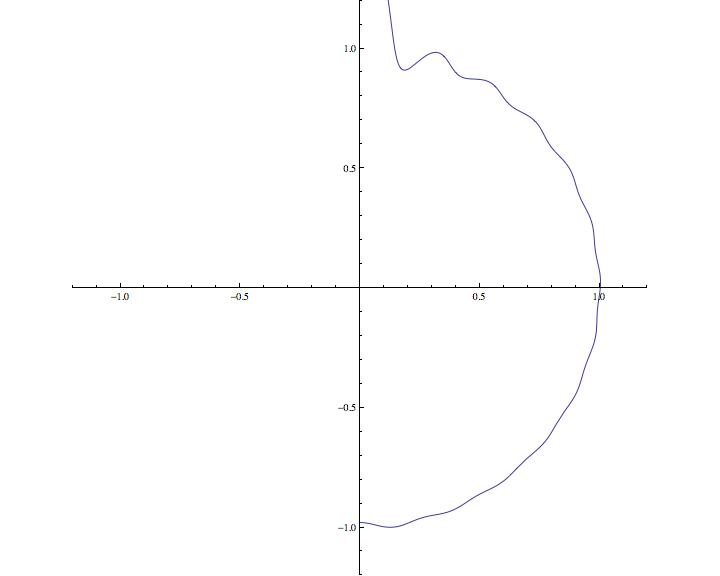
\includegraphics[width=\hsize]{../common/graphics/tsunami0}
\end{center}
\caption{Approximate solution for $N=25$ and $t=0$\label{tsunami0}}
\end{figure}
\begin{figure}
\begin{center}
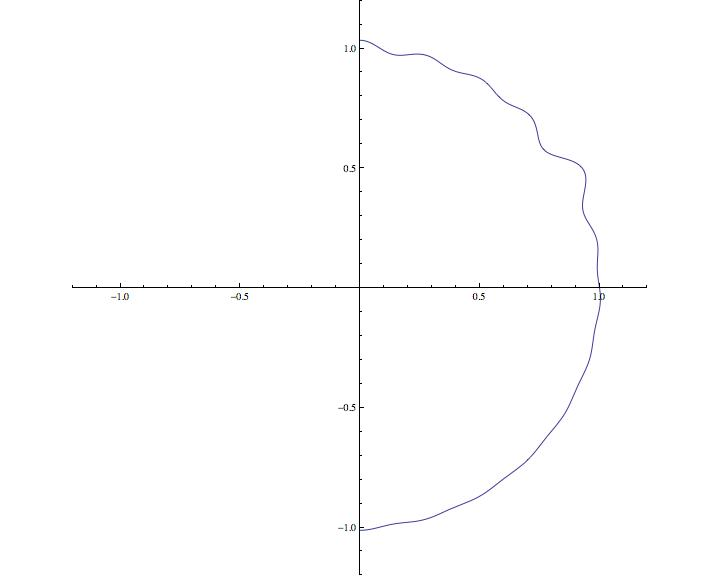
\includegraphics[width=\hsize]{../common/graphics/tsunami50}
\end{center}
\caption{Approximate solution for $N=25$ and $t=1$\label{tsunami50}}
\end{figure}
We now choose initial conditions that are supposed to approximate
what happens for an earthquake.
In a small neighborhood, the function is very large, but zero everywhere
else, but there is no initial velocity.
Thus we postulate that
\begin{align*}
f_\varepsilon(x)&=\begin{cases}
\frac1{\varepsilon}&\qquad 1-\varepsilon<x\le 1\\
0&\qquad\text{sonst}
\end{cases}
\\
g(x)&=0
\end{align*}
This allows to compute the coefficients.
The $b_k$ vanish, only the $a_k$ remain to be computed:
\begin{align*}
a_k(\varepsilon)&=\frac{2k+1}{2}\int_{-1}^1P_k(x)f_\varepsilon(x)\,dx
\\
&=\frac{2k+1}{2}\int_{1-\varepsilon}^1P_k(x)\frac1{\varepsilon}\,dx
\end{align*}
We are mainly interested in the situation where $\varepsilon$ is
very small, so we take the limit $\varepsilon\to 0$
\begin{align*}
\lim_{\varepsilon\to 0} a_k(\varepsilon)
&=
\frac{2k+1}{2}\lim_{\varepsilon\to 0}\frac1{\varepsilon}\int_{1-\varepsilon}^1P_k(x)\,dx
\end{align*}
Using the antiderivative $I_k(x)$ of $P_k(x)$ this becomes
\begin{align*}
\lim_{\varepsilon\to 0} a_k(\varepsilon)
&=
\frac{2k+1}{2}\lim_{\varepsilon\to 0}\frac{I_k(1)-I_k(1-\varepsilon)}{\varepsilon}
\\
&=\frac{2k+1}{2}I_k'(1)=\frac{2k+1}{2}P_k(1)=\frac{2k+1}{2}
\end{align*}
Formally, the solution thus is
\begin{equation}
u(t,x)
=
\sum_{k=0}^\infty \frac{2k+1}{2}P_k(x) \cos \sqrt{k(k+1)}t.
\end{equation}
Unfortunately, this series does not converge, which is not too
surprising given the very special initial conditions.
If we take only $N$ terms and renomarmlize with the factor $\frac1{N^2}$,
we get an approximate idea for the wave propagation.
Figures \ref{tsunami0} and \ref{tsunami50} show the series terminated 
after $25$ terms.
